\chapter{Theoretical background}

\section{Tracking}
\hspace{0.5cm}Video tracking or object tracking in a images sequence is the process of estimating the trajectory of a moving object or various objects time by time in videos or images sequences recorded by a camera or multiple cameras. Tracking action of object can be done by continuously localizing the object with information about regions, points or features of objects in images.\par
Video tracking is widely applied in many fields: human-computer interaction, security and surveillance, traffic control. Many tracking methods have been proposed to tackle the tracking problems, namely, Kalman filter, KCF, CSRT...etc. In pedestrian tracking, the trajectories of the pedestrian are almost predicable and and the velocity is not varied to much or more generally, it can be called a dynamic linear model. Due to the predicting performance in the dynamic linear model and the simple implementation. I decided to use filter as the tracker in my project. The following section briefly describes about Kalman filter.
\pagebreak
\subsection{Kalman filter}
\hspace{0.5cm}The Kalman filter is an algorithm allowing accurate inference in a linear dynamical system, where the state space of the latent variables is continuous and where all latent and observed variables have a Gaussian distribution.\cite{Kalman}

\begin{figure}[h!]
        \centering
        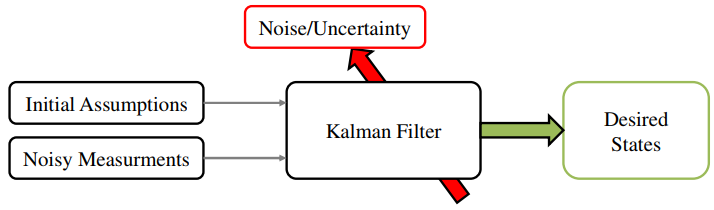
\includegraphics[width=\textwidth]{Chapters/Fig/kalman_dig.png}
        \caption{Diagram of Kalman filter}
        \label{fig:kalman_dig}
\end{figure}\par
Diagram of Kalman filter in fig.\ref{fig:kalman_dig} shows the goal of the filter is to take in impefect information sort out the useful parts of interest, and to reduce the uncertainty or noise.\\
The Kalman filter model assumes that the state of a system that at a time $t$ derived from the prior state at the time $t-1$ defined by the following equation:
\begin{equation}
 \textbf{x}_t = \textbf{F}_t \textbf{x}_{t-1} + \textbf{B}_t \textbf{x}_t + \textbf{w}_t,
\end{equation}\par
where
\begin{itemize}
    \item $\textbf{x}_t$ is the current state vector containing the parameters of interest of the system (e.g, position, velocity, accelerant..) at time t
    \item $\textbf{u}_t$ is the vector containing control inputs
    \item $\textbf{F}_t$ is the state transition matrix which applies the effect of each system state parameters at time $t-1$ on the system state at time $t$
    \item $\textbf{B}_t$ is the control input which applies the effect of each control input parameter in the control input vector $\textbf{u}_t$ on the state vector
    \item $\textbf{w}_t$ is the vector containing the process noise terms fro each parameter in the state vector.
\end{itemize}
\pagebreak
\hspace{0.5cm}Measurements of the system is defined as follow:
\begin{equation}
         \textbf{z}_t = \textbf{H}_t\textbf{x}_t + \textbf{v}_t,
\end{equation}

\hspace{0.5cm}where:
\begin{itemize}
    \item $\textbf{z}_t$ is the vector of measurements
    \item $\textbf{H}_t$ is the transformation matrix that maps the state vector parameters into the measurement domain
    \item $\textbf{v}_t$ is the vector containing the measurement noise terms for each observation in the measurement vector
\end{itemize}\par
There is no direct observation of the true state $\textbf{x}_t$ of the system, and the Kalman filter provides an algorithm to estimate $\hat{\textbf{x}}_t$ using combination of models the system and noisy measurements. Hence, for now, the terms in interest in the state vector are distributed by Gaussian probability density functions (pdfs) rather than discrete values. Gaussian pdfs come up a co-variance matrix $\textbf{P}_t$ which has the diagonal containing the variances associated with the corresponding terms in the state vector and the remaining containing the co-variance between terms in the state vectors.\\
In the prediction state, initial state estimate, $\hat{\textbf{x}}_0$ and $\textbf{P}_0$ are applied recursively at each time step, using a loop then the current state vector is predicted from the state dynamic equation defined as:
\begin{center}
    $
        \hat{\textbf{x}}_{k|k-1} = \textbf{F}_{k-1}\hat{\textbf{x}}_{k-1} + \textbf{G}_{k-1}\textbf{u}_{k-1}, 
    $
\end{center}
\hspace{0.5cm}where:
\begin{itemize}
    \item $\hat{\textbf{x}}_{k|k-1}$ is the predicted state vector
    \item $\hat{\textbf{x}}_{k}$ is the previous estimated state vector
    \item $\textbf{u}$ is the input vector
    \item $\textbf{F}$ and $\textbf{G}$ are the matrices defining the system dynamics
\end{itemize}
\pagebreak
\hspace{0.5cm}Then we predict the state error co-variance matrix by following:
\begin{equation}
          \textbf{P}_{k|k-1} = \textbf{F}_{k-1}\textbf{P}_{k-1}\textbf{F}^T_{k-1} + \textbf{Q}_{k-1}, 
\end{equation}

where:
\begin{itemize}
    \item $\textbf{P}_{k|k-1}$ is the predicted state error co-variance matrix
    \item $\textbf{P}_{k-1}$ is the previous estimated state error co-variance matrix
    \item $\textbf{Q}$ is the process noise co-variance matrix.
\end{itemize}\par
One the predicted valued are obtained, the Kalman gain matrix, $\textbf{K}_k$ is calculated by the following function:
\begin{equation}
              \textbf{K}_k = \textbf{P}_{k|k-1} \textbf{H}^T_k(\textbf{H}_k\textbf{P}_{k|k-1} \textbf{H}^T_k + \textbf{R}_k)^{-1},  
\end{equation}

with $\textbf{R}$ is the measurement noise co-variance.\par
The measurement update equations:
\begin{itemize}
    \item The state vector is updated as:
        \begin{equation}
                      \hat{\textbf{x}}_k = \hat{\textbf{x}}_{k|k-1} + \textbf{K}_k(\textbf{z}_k - \textbf{H}_x\hat{\textbf{x}}_{k|k-1}), 
        \end{equation}
    \item The state error co-variance is updated by
        \begin{equation}
                      \textbf{P}_k = (\textbf{I} -  \textbf{K}_k\textbf{H}_k)\textbf{P}_{k|k-1}, 
        \end{equation}
\end{itemize}
\pagebreak
\hspace{0.5cm}The workflow of Kalman filter is described in this the figure below:
\begin{figure}[h!]
    \centering
    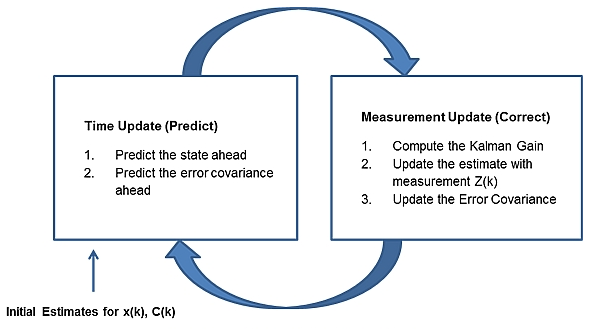
\includegraphics[scale=0.7]{Chapters/Fig/kal_dig_2.png}
    \caption{Workflow of Kalman filter}
    \label{fig:kalman_wf}
\end{figure}
\par
In fig.\ref{fig:kalman_wf}, two states "Predict" and "Correct" of Kalman filter occur continuously with the output of system in the time $t$ is the input of system in the time $t+1$, except the initial time $t_0$. The efficient recursive functions minimize the mean of the squared error in order to provide an optimal status of the model. In several respects, the filter is very powerful: it supports estimates of past, present, and even future states, and it can do so even if the model system's precise nature is unknown.

\section{Deep Learning}
\subsection{Neural Networks}
\hspace{0.5cm}A neural network is a set of algorithm that attempt to expose the underlying relationships in data set through a process that inspired by the way human brain operates. A neural network is a combination of a set highly interconnected computational unit called \textit{neurons}. The diagram below shows a comparison of structure between a biological neural (left) and a neurons in neural network.
\begin{figure}[h!]
    \centering
    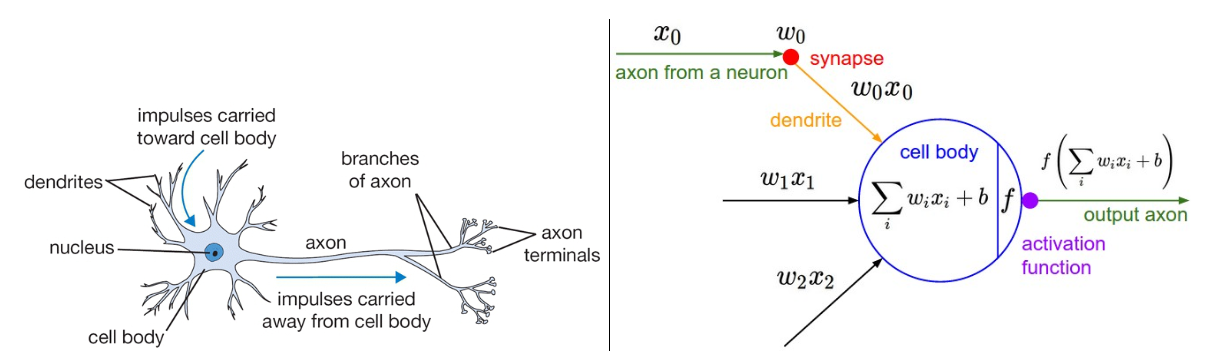
\includegraphics[width=0.9\textwidth]{Chapters/Fig/neural_arc.PNG}
    \caption{Biological neural (left) and a neurons in Neural Network (right) by CS231n course}
    \label{fig:nn_arc}
\end{figure}
Biological neural receives signal for its denrites and generate the output signals onward its axon. In the mathematical neuron unit, input $x_0$ for other neuron combines multiplicatively (e.g $w_0x_0$ )with the dendrites based on the synaptic strength (e.g $w_0$) corresponding to that synapse.\\
In neural network, synaptic strength $w$ can be updated to control the influence strength of input from another neurons in neural network. The activation function $f$ controls the input by calculated a weighted sum of input, add bias and decides whether is should be fired or not.
\subsubsection{Activation functions}
\begin{itemize}
    \item \textbf{Sigmoid} a non-linearity function defined as $\sigma(x)=\frac{1}{1 + e^{-x}}$ with diagram in fig.\ref{fig:sigmoid}. This function normalizes the input to range between [0,1]. Sigmoid is used to be frequently used but rarely now because of two major drawbacks: saturating, killing the gradients and not zero-centered outputs.\\
    \begin{figure}[h!]
        \centering
        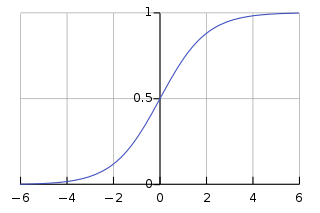
\includegraphics[width=0.4\textwidth]{Chapters/Fig/sigmoid.png}
        \caption{The logistic curve by Wikipedia}
        \label{fig:sigmoid}
    \end{figure}\\
    The derivative of sigmoid function is calculated as:
    \begin{center}
        \begin{equation}
            \begin{split}
                \frac{d\sigma(x)}{dx} & = (\frac{1}{1+e^{-x}})^2\frac{d}{dx}(1+e^{-x})\\
                                    & = (\frac{1}{1+e^{-x}})(\frac{e^{-x}}{1+e^{-x}})\\
                                    & = [1-\sigma(x)]\sigma(x)
            \end{split}
        \end{equation}
    \end{center}
    \pagebreak
    \item \textbf{Tanh} a non-linearity hyperbolic function that squashes a real number to the range [-1,1]. It zero-centers the output, however,it also saturate the gradients as Sigmoid activation function. The tanh function is defined as:
    \begin{equation}
        \text{tanh}(x) = \frac{e^x - e^{-x}}{e^x + e^{-x}} = 2\sigma(2x) - 1
    \end{equation}
    with the derivative is computed as:
    \begin{equation}
        \frac{d\text{tanh(x)}}{dx} = 1-\text{tanh}^2(x)
    \end{equation}
    The graph of the tanh activation function shown in fig.\ref{fig:tanh}
    \begin{figure}[h!]
        \centering
        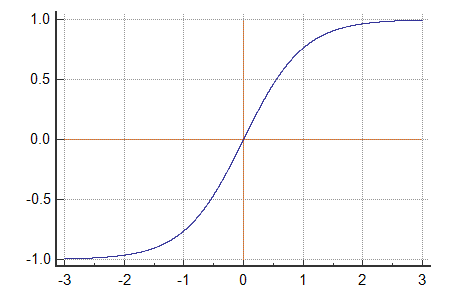
\includegraphics[width=0.4\textwidth]{Chapters/Fig/tanh.png}
        \caption{Tanh activation function}
        \label{fig:tanh}
    \end{figure}

    \item \textbf{ReLU} The Rectified Linear Unit graph of which shown in fig.\ref{fig:relu} computes 
    \begin{equation}
        f(x) = max(0,x)
    \end{equation}
    It has been widely used in the last few years because it more highly accelerates the convergence of stochastic gradient descent than sigmoid/tanh functions due to its linear, non-saturating form. Moreover, implementation of ReLU is easier than sigmoid/tanh functions by simply thressholding a matrix of activations at zero. However, ReLU units can be fragile during training and can die [cs231n]
    \begin{figure}[th!]
        \centering
        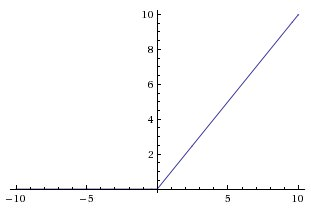
\includegraphics[width=0.4\textwidth]{Chapters/Fig/relu.jpg}
        \caption{The graph of ReLU}
        \label{fig:relu}
    \end{figure}\\
    The derivative of ReLU is:
    \begin{equation}
        \frac{df}{dx} = \begin{cases}
            1 & x < 0\\
            0 & \mbox{otherwise}
        \end{cases}
    \end{equation}
    \item \textbf{Leaky ReLU} is proposed to fix the "dying ReLU" by having a small slope for negative values instead of zero.
        \begin{equation}
        \frac{df}{dx} = \begin{cases}
            1 & x < 0\\
            \alpha x & \mbox{otherwise}
        \end{cases}
    \end{equation}
    where $\alpha$ is a small constant
    \begin{figure}[h!]
        \centering
        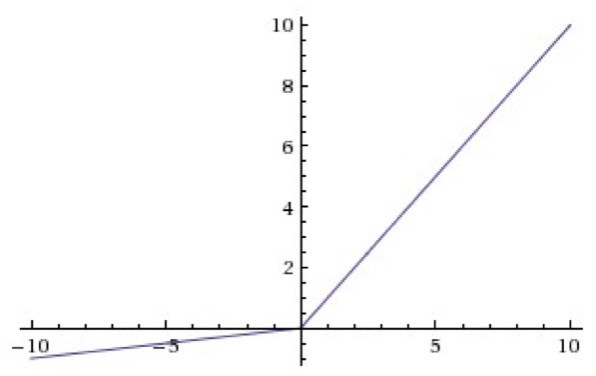
\includegraphics[width=0.4\textwidth]{Chapters/Fig/leaky.jpeg}
        \caption{The graph of Leaky ReLU}
        \label{fig:lrelu}
    \end{figure}
\end{itemize}

\subsection{Deep Forward Networks}
\hspace{0.5cm} Deep forward networks or feedforward neural networks or multilayer perceptrons are the foundation of most deep learning models. The main goal of feedforward network is to approximate some function $f*$. For example, for a regression, $y = f*(x)$ maps an input x to a value y. A feedforward network defines a mapping $y = f(x;\theta)$ and learns the value of the parameters $\theta$ that result in the best function approximation.\par
These model are called feedforward since the data runs through the mapping from $x \rightarrow y$ to define $f$ without any feedback connections in which outputs of the model are fed back into itself. In a special case, there exists feedback connections in the network, they are called recurrent neural networks which is not presented in this work.
\pagebreak
\subsubsection{The architecture}
\hspace{0.5cm} The architecture of the structure of the network refers to the number of hidden layers and the number of hidden units or neurons in each layer. The term network in the name of these models means that they can be represented as a combination of many different functions. For example, suppose we have 3 functions $f^{(1)}$, $f^{(2)}$ and $f^{(3)}$ connected into a chain to form the mapping $f(x) = f^{(3)}(f^{(2)}(f^{(1)}(x))$. In this example, $f^{(1)}$ is called the first layer of the network, $f^{(2)}$ is called the second layer and so on. The final layer is called output layer while the layers between the input and output layers are called hidden layers because the training data does not show the desired output for each of these layers. The length of the chain defines the depth of the network
\begin{figure}[h!]
    \centering
    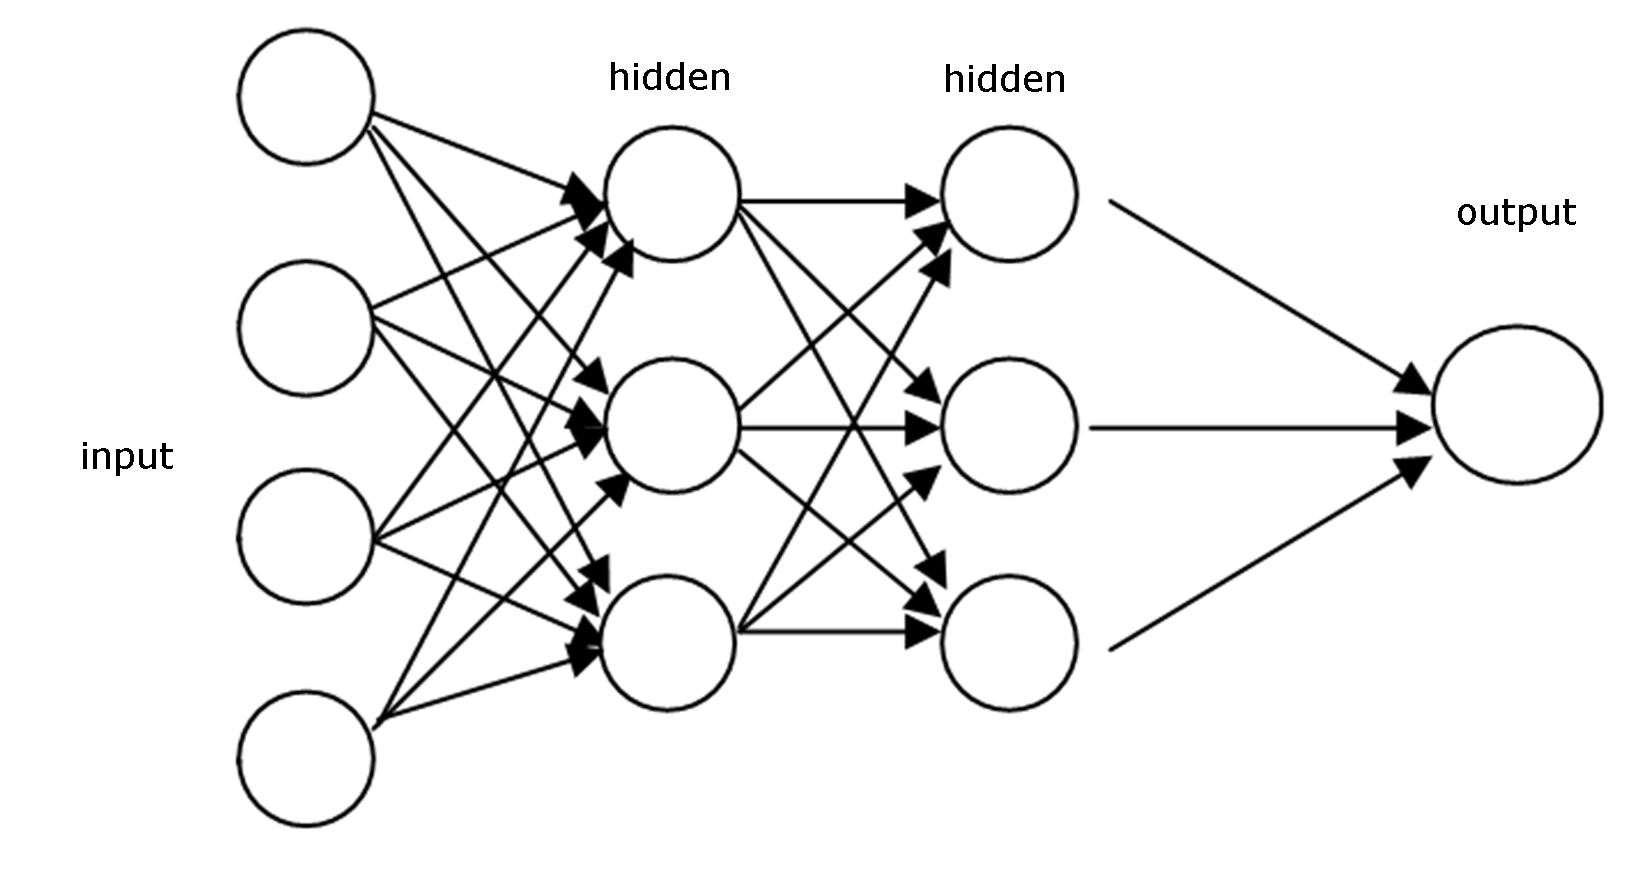
\includegraphics[width=0.6\textwidth]{Chapters/Fig/architecture_mlp.png}
    \caption{Architecture of a simple feedforward neural network}
    \label{fig:arch_mlp}
\end{figure}
\par Fig.\ref{fig:arch_mlp} describes a architecture of a simple feedforward neural network which has two hidden layers which 3 nodes for each hidden layers.






\pagebreak
\section{Object Detection}
\subsection{Intersection over Union (IoU)}
\hspace{0.5cm}Intersection over Union (IoU) is the ratio of overlapping area of predicted bounding box and the ground truth bounding box over the total area of the both boxes. This metric allows us to evaluate how well the detector predict the bounding box of the object comparing to the ground truth ones.
\begin{figure}[h!]
    \centering
    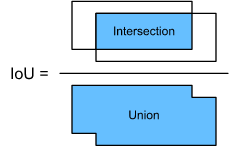
\includegraphics[scale=1]{Chapters/Fig/iou.png}
    \caption{Intersection over Union}
    \label{fig:iou}
\end{figure}\par

Ideally, if the predicted and the ground truth bounding boxes overlapped perfectly, the IoU would be equal to 1. However, in practical, the IoU greater than or equal to 0.5 is good to be used as threshold to determine the predicted bounding box is correct or not.
\subsection{Non-maximum Suppression}
\hspace{0.5cm}One the problems of Object Detection is that the algorithms may output multiple detections for the similar objects in multiple times. Non maximum suppression is an approach to make sure that a particular in the image scenes is identified only once.
\begin{figure}[h!]
    \centering
    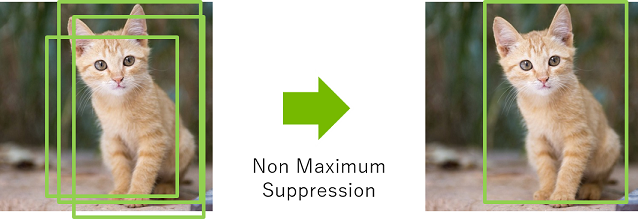
\includegraphics[width=0.8\textwidth]{Chapters/Fig/nms.png}
    \caption{Non Maximum Suppression}
    \label{fig:nms}
\end{figure}\par
For example, in the fig.\ref{fig:nms}, the algorithm may output a lot of detections with different confidence score (is a cat or not), then we run the these detections through our non maximum suppression which will get rid of boxes which have lower confidence scores and keep the only one bounding box with the highest confidence score.
\pagebreak
\subsection{Anchor box}
\hspace{0.5cm}Anchor boxes are the set of predefined height and width bounding boxes which are used for assist the algorithm to be more certain in training and give the algorithms ability to detect more precise.
In real life, the bounding boxes of the objects are not arbitrary. Cars, vans have similar shapes of bounding box with larger width than height while pedestrian have an approximate aspect ratio of 0.41.
\begin{figure}[h!]
    \centering
    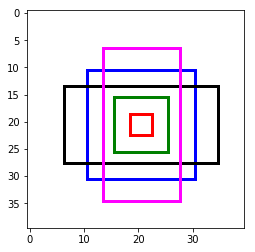
\includegraphics[scale=0.5]{Chapters/Fig/anchor_boxes.png}
    \caption{5 anchor boxes}
    \label{fig:ab}
\end{figure}\par
Moreover, instead of predicting absolute value of bounding boxes such as $x,y,w,h$ or $x1,y1,x2,y2$, the algorithms now only predict offsets corresponding to each of the anchor boxes . If we normalize the offset values in a fixed range, we can maintain the diversity, therefore, the initial training will be more stable.
